With new devices constantly being designed and fabricated, new avenues being probed, the structure of experiments can become convoluted. The needless post-processing of all acquired data to top it all off is \todo[inline]{gargghh}


The apparatus I am applying my work to is by no means comprehensive, but it serves as a reference point in a proven device. To accomplish this body of work with this particular device would 


Figure \ref{fig::set_layout} \cite{morello2010single}
shows the physical device that will be similar to one I will be testing my solution on. This devices has various control points, such as the top gate to induce a layer of electrons on the boundary, the left and right barriers to remove this layer, forming tunnel junctions to the island, and finally the plunger to control the gate, as in a MOSFET.
\subsection{Problem Statement}
\todo[inline]{Say something5}

\begin{figure}[htbp!]
	\centering
	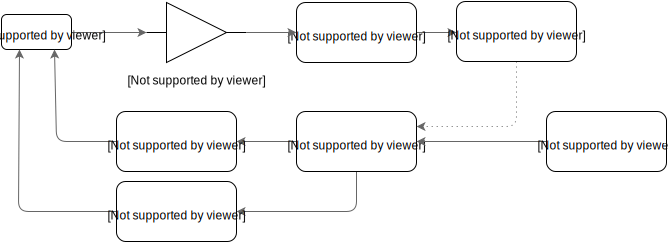
\includegraphics[width=\textwidth]{thesis_experiment.pdf}
	\caption{Block diagram of experiment}
	\label{fig::thesis_experiment}
\end{figure}

\subsection{Digital Devices}
\subsubsection{PCIe Digitizer Card}
\todo[inline]{Talking points of the Digitizer solution, DMA, etc. etc.}
The ATS9440 \gls{pcie} digitizer card \cite{ATS9440} has been incorporated into the previous years' research and hence, a lot of the groundwork has been laid out for using the device, and interfacing it with experiments. It is the natural solution, to attempt to provide digital feedback in a MATLAB environment in a semi-real-time capacity. There is a clear benefit in utilizing what is already well established, conditional that it can achieve what is necessary.

The primary features of this solution are:
\begin{itemize}
	\item Range of sampling frequencies from 1 KS/s to 125 MS/s
	\item 4 independent input channels
	\item Internal (from one of the 4 input channels) and external triggering
	\item 14-bit resolution, with definable input ranges of $\pm 100 \textrm{mV}$ to $\pm 4 \textrm{V}$
	\item Auto-\gls{dma} for fast storage and parallel data processing.
\end{itemize}

\subsubsection{FPGA/$\mu$Controller and ADC}
\todo[inline]{Talking points of the external FPGA and ADC solution, mention some particular examples of ADCs etc.}
An alternative solution is to have an external device which is responsible for detecting peaks in the \gls{set} current, and waiting a predetermined amount of time before setting a TTL output to high, which could then trigger the plunge, and the experiment to begin.

This approach requires the design of a high precision \gls{adc}, with a sampling rate of at least 1 MS/s. The digital data would then need to be processed by either a $\mu$Controller or a \gls{fpga}. The primary benefit of this solution is that it is versatile, and can be adapted and modified to meet different needs of the future. Furthermore, as this is completely external to the rest of the experiment, it can truly run in parallel, and accurate timing without error could prove to be more achievable.
\subsubsection{XMC}
\todo[inline]{Talking points of the integrated XMC solution, pre-built FPGA, ADCs and possibly with Auto-DMA}

\begin{figure}[htbp!]
	\centering
	\includegraphics[width=\textwidth]{set_layout}
	\caption{The layout of an SET}
	\label{fig::set_layout}
\end{figure}